\chapter{Diagrammes}
\label{s:Diagrammes}


\section{Diagramme de contexte}
\label{s:Diagramme_contexte}

\begin{figure}[htp]
   \centering
   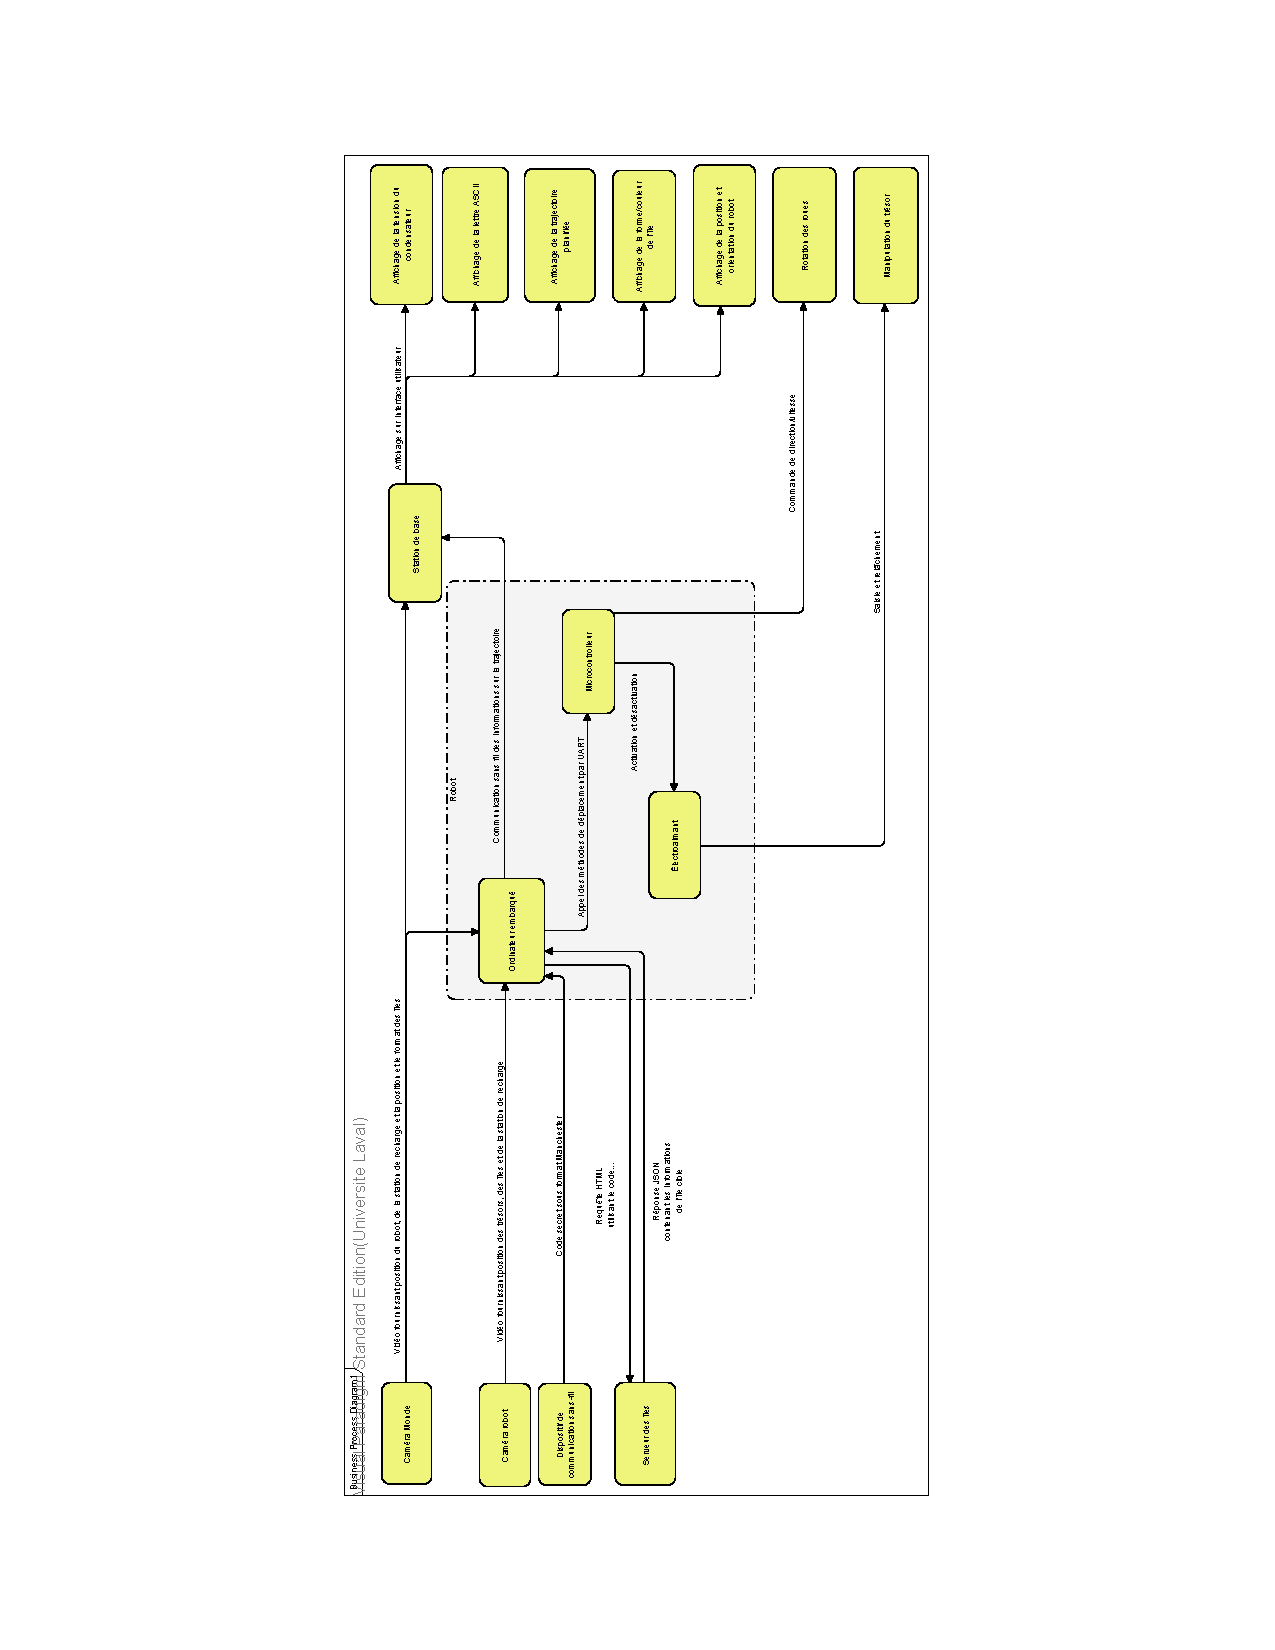
\includegraphics[width=0.75\textwidth, angle =-90]{pdf/ContextDiagram.pdf}
   \caption{Diagramme de contexte}
   \label{f:Diagramme_contexte}
\end{figure}

\newpage

\section{Diagramme de classes}
\label{s:Diagramme_classes}

\begin{figure}[htp]
   \centering
   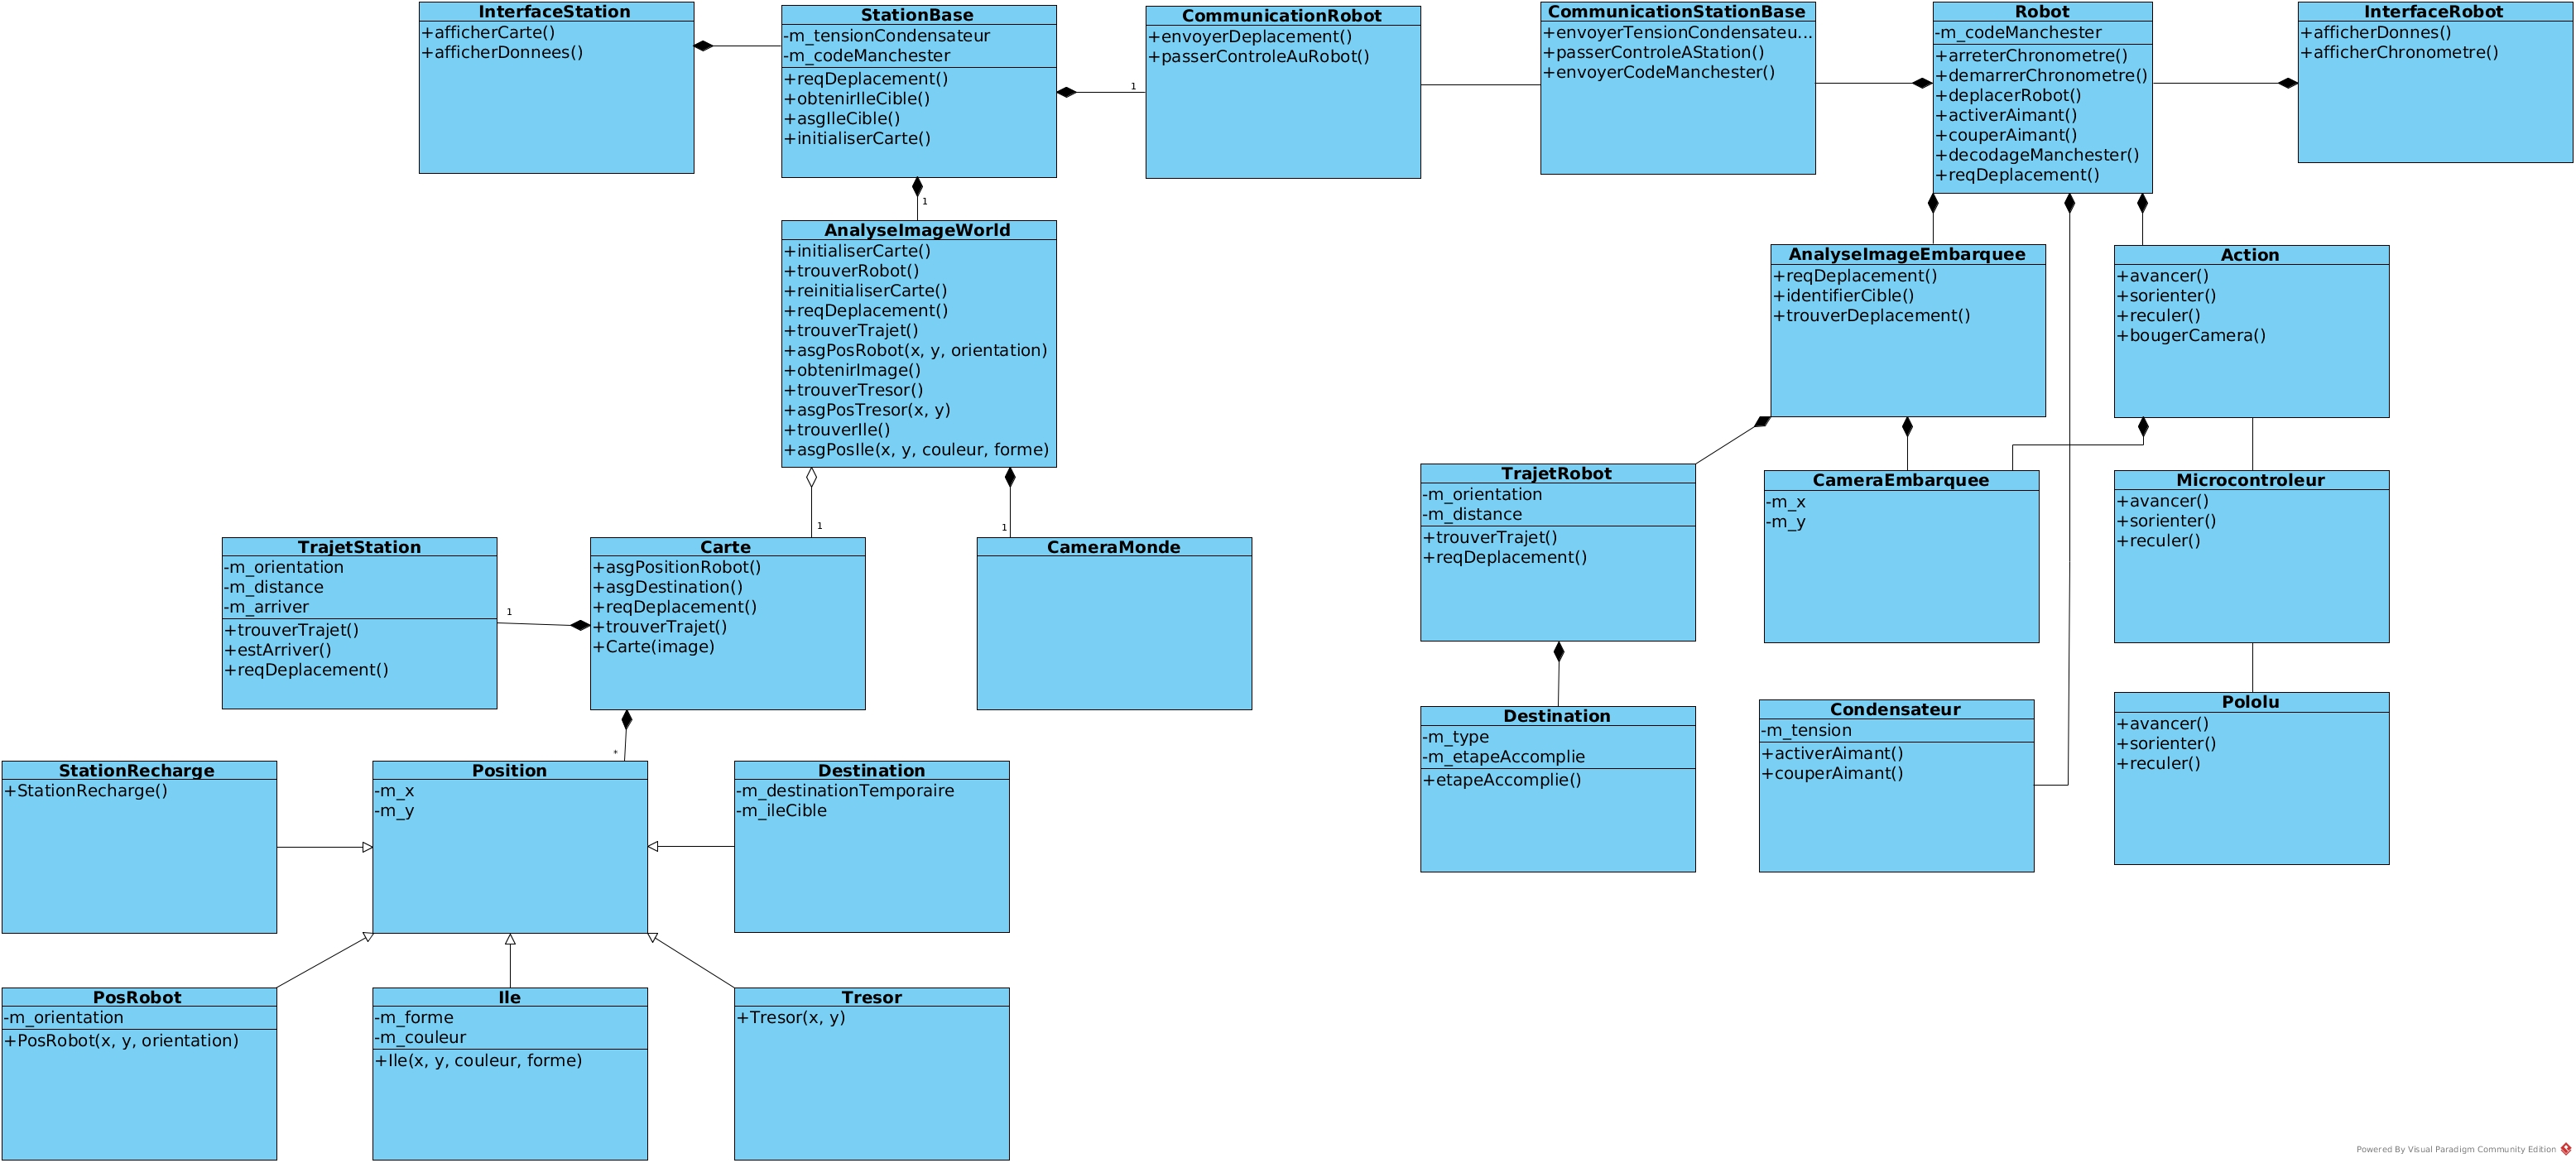
\includegraphics[width=0.95\textwidth, angle =-90]{fig/ClassDiagram.jpg}
   \caption{Diagramme de classes}
   \label{f:Diagramme_Classes}
\end{figure}

\newpage


La figure \ref{f:Diagramme_Classes} repr�sente le diagramme de classes suite � la premi�re it�ration. La structure est suseptible de changer suite aux prochaine it�rations, mais voici une br�ve description de la structure sur laquelle nous nous entendons pr�sentement. \par

La section de gauche du diagramme sera impl�ment�e sur la station de base tandis que la section droite sera impl�ment�e sur le robot. Ces deux syst�me pouront communiquer entre eux � l'aide des classes CommunicationRobot et CommunicationStationBase. \par

En ce qui conscerne la station de base, le contr�leur du syst�me est repr�sent� par la classe StationBase. La classe AnalyseImageWorld analyse les images re�u de la CameraMonde et g�n�re une carte sh�matique de la table (Carte) � l'aide d'imagerie. La carte est compos�e de diverses �l�ments qui h�rite tous de la classe Position. Les trajectoires du robot seront calcul� dans la classe TrajetStation � l'aide des informations de la classe Carte.  \par

Pour ce qui est du robot, il est aussi compos� d'un contr�leur (Robot). Les mouvements que devra effectuer le robot passerons tous par la classe Action qui les acheminera au microcontroleur et au polulu si nescessaire. Lorsque le robot est pr�s de la destination, TrajetRobot calculera les trajets (� l'aide de Destination et d'imagerie effectu� dans AnalyseImageEmbarquer).

    
   



\section{Diagramme de s�quences}
\label{s:Diagramme_sequences}

\begin{figure}[htp]
	\centering
	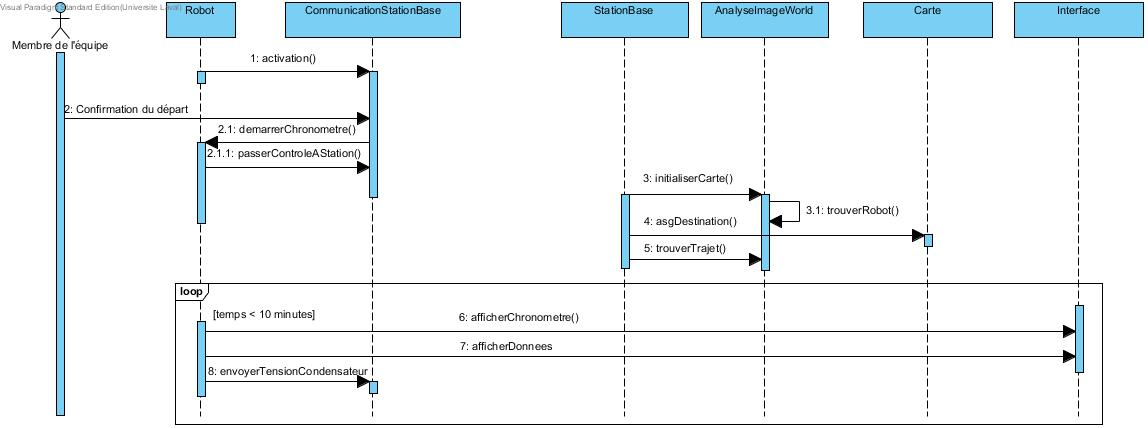
\includegraphics[width=0.95\textwidth]{fig/demarrageRobot.jpg}
	\caption{D�marrage du Robot}
	\label{f:DemRob}
\end{figure}

%\begin{figure}[htp]
%   \centering
%   \includegraphics[width=1\textwidth]{Diagramme_sequences}
%   \caption{Diagramme de s�quences}
%   \label{f:Diagramme_sequences}
%\end{figure}

